\chapter{Tellervo-lite}
\label{txt:tellervolite}

Tellervo-lite is the form that the Tellervo desktop application takes when you disable integration with the Tellervo server.  The basic interface of Tellervo-lite is very similar to the full Tellervo, however, it lacks many of the advanced features such as 3D mapping, curation, and metadata management.  If you are looking for a easy to use tool for simply measuring dendro samples and editing existing data files, then Tellervo-lite may be the best option for you.

Tellervo-lite is a `mode' of the standard Tellervo application, not a smaller separate application.  There is a unified installation procedure for installing Tellervo, and the switch to `lite' mode is done during the configuration stage the first time you launch the application.  If you have not installed Tellervo yet, please do so now by following the instructions on page \pageref{txt:desktopinstall}.

\section{Launching Tellervo-lite}
The first time you launch Tellervo you will be presented with the setup wizard.  The first question asks whether you'd like to use the standard Tellervo or Tellervo-lite.  If you have decided to convert to Tellervo-lite mode at a later date (or vice versa), you can make the change by going to \menutwo{Help}{Setup wizard} to relaunch the wizard, or by going to \menutwo{Edit}{Preferences} and ticking the `disable databse integration' checkbox on the network tab.  Once you have launched (or relaunched) Tellervo in lite mode you will see the main screen shown in figure \ref{fig:tellervolitehome}.

\begin{figure}[hbtp]
  \centering
    
\includegraphics[width=0.8\textwidth]{Images/tellervolite.png}
  \caption{The main screen when Tellervo is launched in lite mode.}
  \label{fig:tellervolitehome}
\end{figure}

\section{Tellervo-lite interface}

The main Tellervo-lite interface is split into two parts.  On the left is the series list, which contains all of the measurement series present within the current data file.  On the right are two tabs: the data tab which contains the ring measurement values table and a graph representation; and the metadata tab which contains some basic metadata fields.  Depending on the file format you intend to use, the series list may have one or more measurement series.  For instance the Tucson RWL data format is capable of storing multiple series, whereas the Sheffield format can contain just one.

\subsection{Data tab}

The data tab contains three main panels: data table; graph; and remarks panel, all out which can be resized to suit your needs.  The remarks panel enables you to tag individual rings with features, however, there is currently no support for saving this information in legacy files so it's not particularly useful in the context of Tellervo-lite and is therefore collapsed by default.  The data table provides a way to view and edit the ring width data for your series, and is arranged in decades.  You can enter and edit data within the table directly by clicking the cell and typing in a value.

The graph panel shows a basic chart of the ring width data and has it's own toolbar for adding/removing features, zooming etc.

At the bottom of the data tab is a status bar providing some summary information about the series.  It includes: the calendar being used (whether absolute or relative); year and size of the currently selected ring; the variable being displayed (whole ring width; early/latewood width etc); the current measurement units; and some basic statistic.  Clicking on the final three items, gives you options to change what is displayed.


\subsection{Metadata tab}

The metadata tab in Tellervo-lite provides a very generic and simplified method for entering the most common metadata to legacy dendro data files.  The type of metadata stored in legacy data formats varies substantially, from essentially none (e.g. Belfast format) to quite rich (e.g. Heidelberg format).  The time it would take to provide, maintain and support a metadata screen tailored to each format would be prohibitive.  Besides, if you are interested in storing rich dendro metadata you should really be using the full version of Tellervo!  The metadata screen in Tellervo-lite therefore provides the ability to add/edit a few of the very core metadata fields supported by most data formats.

At the top of the metadata tab is a pull down menu for specifying how the series are grouped.  This is only relevant if you have multiple series in your file but will affect how the metadata fields behave and how files are saved depending on the output format you choose.  For example, if you specify that the series are all from the same site/object, then then site/object name will be syncronised across all the series.  Similarly, if the series are from the same tree, then the species field will be synchronised.  If you choose to save a to a file format that expect all series to be from the same site, yet you specify the series are from different sites, then Tellervo will save each series to a separate file.


\section{Measuring a new sample}

To begin measuring a new sample you should start by clicking the \menutwo{File}{New} menu or by clicking the corresponding button on the toolbar.  A new `Untitled' series will appear in your sample list.  Next, switch to the metadata tab and enter the name for this series and any other of the metadata fields that are desired.  You can now switch back to the data tab.  You can add as many series as you like by clicking the add series button at the top of the series list.  You can also sort the series using the drop down menu at the bottom of the panel.

Before you begin measuring you need to tell Tellervo what sort of measurements you are making: whole ring widths; or early/latewood widths (the default is whole ring widths).  To specify early/latewood widths you need to go to \menuthree{Edit}{Measuring mode\ldots}{Early and latewood widths}.  If you use this menu after you have already measured some rings you will be warned that Tellervo will delete the data you have already collected.  Once in `early and latewood widths' measuring mode you will be able to choose which data is displayed in the table by clicking the variable box on the status line and choose between: Ring width; Earlywood width; Latewood width; Early/Latewood width.

To begin measuring your sample you can now go to \menutwo{Edit}{Start measuring}, press the start measuring button on the toolbar, or you can press F5. While measuring you should be provided with audible feedback for each ring measured with a more pronounced sound made every 10th ring. If there is a problem communicating with your measuring hardware, check your settings in the preferences dialog. If you still have problems contact the Tellervo developers by going to \menutwo{Help}{Email developers}, making sure you include details of your hardware and any error messages that you receive.

If your sample is already dated and/or you already know how many rings your sample has, then you can initialise your data matrix using the button on the toolbar or the menu item in the edit menu.  This gives you a dialog requesting date and ring number information which can be useful for those of you that use the skeleton plotting method prior to measuring.  

Note by default Tellervo labels rings as relative years beginning in 1001 (a convention from the days of mainframe computers and punchcards).  If your sample is dated, you should explicity tell Tellervo either using the initialise grid function prior to measuring, or by going to \menutwo{Tools}{Redate} once you've finished.

Depending on the measuring platform hardware you have, you will see some variation of the measuring panel in figure \ref{fig:measurepanellite}. The left display holds the absolute position of the last ring boundary (for devices that measure cumulatively), the middle display holds the last recorded measurement width and the right display holds the current position of the measuring plaform (for devices that report live measurements).  The right-hand display is useful for devices that don't have a physical display such as the Lintab. 

\begin{wrapfigure}{r}{0.5\textwidth}
  \begin{center}
    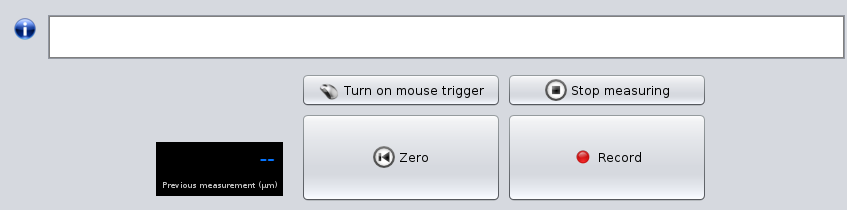
\includegraphics[width=70mm]{Images/measuringpanel.png}
  \end{center}
  \caption{Measuring control panel.  The number of digital displays will vary between 1 and 3 depending on what type of measuring platform hardware you have.}
  \label{fig:measurepanellite}
\end{wrapfigure}


Tellervo supports the measuring of rings both individually and cumulatively.  We feel that it is easier and more accurate to measure rings individually, that is to say the device is reset to zero after each measurement.  If a device accepts requests to reset measurements (e.g.\ Quadra Chek boxes) or if it automatically resets itself to zero after recording a measurement (e.g.\ EVE IO) then this procedure is used by Tellervo.  In this case the user begins measuring by setting the display to zero, then moves the platform to the end of the ring, then either presses the `measure' button on the hardware device or the `record' button on the screen.

\tip{If your device does not have a physical `measure' button you don't need to click on the `record' button each time.  Instead click on the `turn on mouse trigger' button and then you can use your mouse's left button as a measure button regardless of where the mouse is on the screen. This means you don't need to lift your eyes from your microscope to ensure you are clicking the button correctly.  When you're finished measuring press escape to exit this mode.  Alternatively you can use the tab key to ensure the record button has focus and then you can use the spacebar on your keyboard.}

Certain devices (e.g. Boekler Microcode boxes) do not listen for requests to reset to zero.  In this case to measure each ring individually, you would need to manually reset the reading to zero following each measurement.  This would of course be extremely tedious.  In this situation Tellervo measures cumulatively from the beginning of the first ring and calculates the ring width based on the previous ring boundary position.  With this method you must be careful not to knock your sample, and you must also take special care when altering radii to navigate around problem structures.  If you do knock your sample, the best way to recover is to reset your platform to zero and press the measure button.  Next, press the `stop measuring button', manually fix the values in the data table, then begin measuring again from where you left off.

If you are in `Early and latewood widths' measuring mode the measurements are made and sent to the data table in pairs.  The first measurement should be of the earlywood of the ring, and the next value the latewood measurement.  Whether you are currently measuring early or latewood is indicated as a message at the bottom of the measuring panel.


\section{Loading existing files}

If you have existing data files that you would like to examine and/or edit, these can be opened using the \menutwo{File}{Open} menu or the equivalent button on the toolbar.  Through the use of the TRiCYCLE conversion library \citep{tricycle}, Tellervo supports many legacy dendro data formats.  Select the correct format from the format list in the dialog and then select the file you'd like to open.  You can now make changes to the data and/or metadata just as if it was a new series.  Ring width values can be changed manually just by clicking on the value in the table and typing in the new value, or you can use the \menutwo{Edit}{Start measuring} menu to remeasure rings.

\section{Inserting, deleting and remeasuring rings}

If you find you need to insert or delete a ring in your dataset, the easiest thing to do is to right click on the cell in question and use the popup menu.  You can also find similar options in the edit menu.  You will notice that in the popup menu there is also the option of tagging a ring with various features (e.g. frost damage, false ring etc).  This feature exists in Tellervo-lite, however, there is currently no support for saving this information to legacy data files.  

If you want to remeasure a ring (or series or rings) you need simply highlight the ring in the data table and measure as normal.  The new measurements will simply be pasted over the top of the old ones.

\section{Saving}

Saving your changes is simply a matter of going to \menutwo{File}{Save} or \menutwo{File}{Save as}, or using the corresponding toolbar icons.  If you are saving to a new file, then you will need to choose the format you'd like to use from the file save dialog.  There is no need to add the file extension for formats that have a standard extension as Tellervo will automatically add this for you.

If you have loaded an existing data file, you will be warned that overwriting it may result in the loss of some metadata.  If your original file contained metadata not supported by the rudimentary fields in the metadata tab, then this metadata will be missing from the newly saved file.  You may therefore prefer to use the \menutwo{File}{Save as} option and save to a new file instead.

If you have multiple series in your file and you attempt to save to a format that only supports one series per file, Tellervo will warn you and ask whether you'd like to use the keycodes of the series as file names.  If you answer yes the files will be saved within the specified folder with the keycodes as the file names, otherwise it will create a series of files with the same filename with a number suffix.




